\documentclass{article}
\usepackage[utf8]{inputenc}
\usepackage{float}

\title{\textbf{Projeto CE4411:} Jogo memorização de LEDS}
\author{
  ROSA, Vitor Acosta da\\
  \texttt{RA: 22.218.006-9}
  \and
  BARBOSA, Andy Silva\\
  \texttt{RA: 22.218.025-9}
}
\date{14 de Maio de 2020}

\usepackage{natbib}
\usepackage{graphicx}

\begin{document}
\maketitle
\section{Descrição do projeto}
Para o projeto foi escolhido desenvolver um jogo de memorização de LEDS. No qual, foi utilizado o simulador EdSim51 para a criação e execução do código para um microcontrolador 8051.\\
No jogo, o usuário deve memorizar uma sequência aleátoria de LEDS que acendem um de cada vez e apertar os botões na ordem correta para todo LED aceso. Em caso de vitória ou derrota no jogo, o \textit{display} LCD apresentará a mensagem para cada ocorrência, sendo possível começar um novo jogo.
\section{Desenho esquemático}
\begin{figure}[H]
\hspace*{-1.5in}
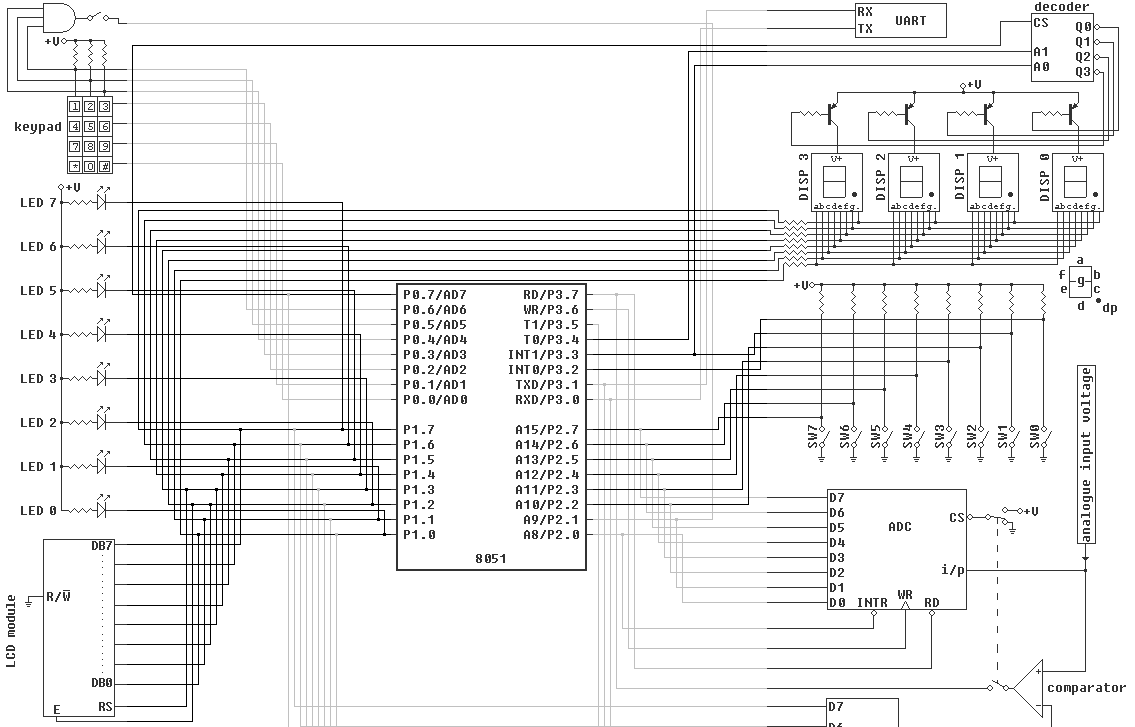
\includegraphics[scale=0.5]{diagrama.png}
\caption{Diagrama esquemático do 8051 para o jogo. Fonte: EdSim51}
\end{figure}
Para o jogo, como mostra a figura 1, foram utilizados somente: o \textit{display} LCD para exibir a condição de vitória ou derrota, o \textit{LED Bank} para acender ou apagar os LEDS de 7 a 2, o \textit{Switch Bank} para a inserção da sequência pelo usuário e o \textit{Multiplexed 7-Segment Display}.\newline
Vale ressaltar que os pinos P3.2 e P3.3 foram definidos como interrupções externas, e ocupam as chaves SW0 e SW1 respectivamente. Por tal fato, ambas as chaves e os LEDS respectivos 0 e 1, não são utilizados na sequência para o jogo, restando os LEDS de 2 a 7 e as chaves de SW2 a SW7.
\newpage


\section{Diagrama}
\subsection{Considerações gerais}
Para que o jogo flua de maneira correta, e que apresente o melhor resultado e jogagabildade possível, é recomendo jogar com a frequência de \textit{update} igual a 8, o que pode ser configurado facilmente no EdSim51, através da opção \textbf{Update Freq.}, como mostra a figura 2.
\begin{figure}[H]
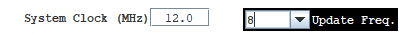
\includegraphics[scale=1]{freq.PNG}
\caption{Configuração geral pré-jogo.}
\end{figure}

\subsection{Utilização das portas}
Para o jogo, as portas foram configuradas da seguinte maneira:
\begin{figure}[H]
\hspace*{-1.5in}
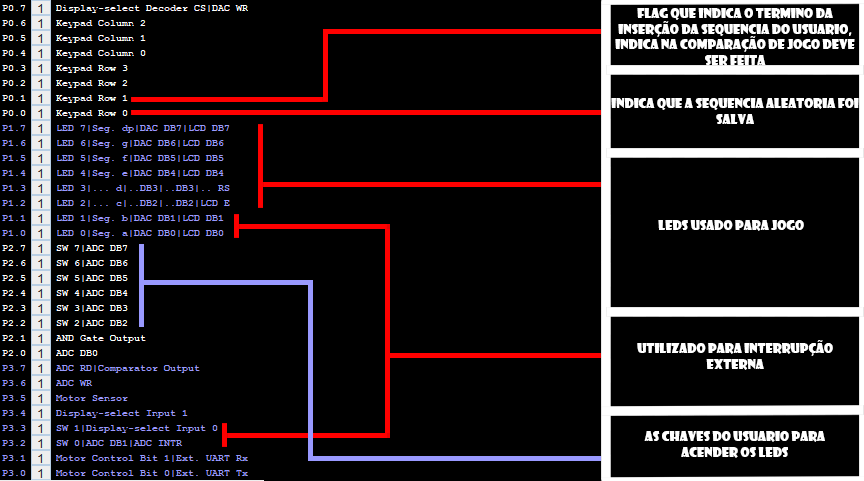
\includegraphics[scale=0.6]{TELA_DAS_FLAGS.png}
\caption{Configuração das portas.}

\end{figure}
\subsection{Uso dos registradores}
\begin{figure}[H]
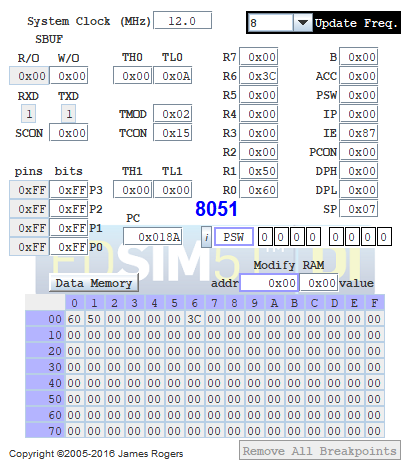
\includegraphics[scale=1]{registradores.PNG}
\caption{Utilização dos registradores. Fonte: EdSim51}
\end{figure}
Configurações dos registradores, dada por:\newline
\textbf{R0 (Espaço de memória 00):} Ponteiro de memória (com o valor inicial 60) para o salvamento da sequência inserida pelo usuário no decorrer do jogo. \newline
\textbf{R1 (Espaço de memória: 01):} Ponteiro de memória (com valor inicial 50) para o salvamento da sequência aleatória gerada pelo algoritmo. \newline
\textbf{R6 (Espaço de memória: 06):} Utilizado para gerar delay, seu valor padrão é dado por $3C_{16}$ ou $60_{10}$.
\newline
Os demais registradores não são utilizados na implementação do jogo. Esses valores são os iniciais, \textit{setados} por uma rotina de pré-jogo.
\subsection{Números aleatórios}
\begin{figure}[H]
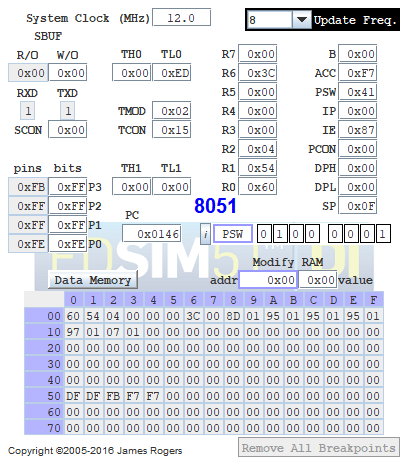
\includegraphics[scale=1]{random.PNG}
\caption{Sequência aleatória de LEDS nas posições de memória 0x50 a 0x54. Fonte: EdSim51}
\end{figure}
No espaço de memória entre 0x50 e 0x54 é salvo a sequência aleatória gerada pelo algortimo.\newline
Tal sequência é gerada em três partes.\newline
\textbf{Rotina "Gera-seed":} A partir do valor disposto no \textit{timer0} (TL0) é calculado um novo valor de recarga para esse \textit{timer}, a fim de quebrar o ciclo e manter a aleatoriedade entre cada LED aceso da sequência.\\ O cálculo da semente é realizado da seguinte maneira: primeiramente, multiplica-se o valor disposto no TL0 por $17_{10}$, em seguida é feita uma rotação de todos os bits para a esquerda, considerando o \textit{carry} nesta operação, como a multiplicação é separada entre MSB (armazenado no registrador B) e LSB (armazenado no acumulador A), a próxima etapa envolve a soma de ambos e para finalizar há a sobreposição do valor de TL0 por essa semente.\newline
\textbf{Rotina "Random":} Essa rotina gera de fato a sequência aleatória de LED.\\Para acender um LED por vez é fornecida uma sequência inicial (dada por $0111111_{2}$, na qual cada número representa um LED). \newline Antes de qualquer cálculo, é chamada a rotina \textbf{Gera-seed}, após isso é movido o valor do contador para o acumulador A, em seguida, é feita a divisão por 6 (por conta dos LEDS que são utilizados no jogo), o resto (armazenado no registrador B) é considerado, e o quociente(armazenado no acumulador A) descartado.\\
Dessa forma, o resto representará a quantidade de vezes que a sequência de 8bits iniciais ($0111111_{2}$) passará na rotina de rotação.\newline
\textbf{Rotina "Rotate":} Rotaciona para a direita a sequência de 8bits calculada na rotina Random disposta no acumulador A, o número de vezes armazenado no registrador B.\newline
Após todo esse processo, é chamada a rotina "Salva-Seq", que, a partir do ponteiro de memória dado pelo registrador R1, armazena a sequência entre as posições 0x50 e 0x54.

\subsection{Números inseridos pelo usuário}
\begin{figure}[H]
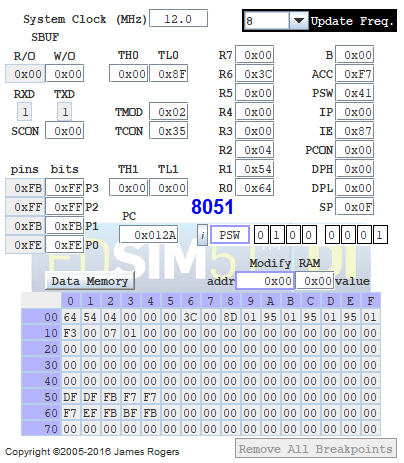
\includegraphics[scale=1]{sequsuario.PNG}
\caption{Sequência de LEDS inserida pelo usuário nas posições de memória 0x60 a 0x64. Fonte: EdSim51}
\end{figure}
Assim que a sequência aleatória gerada pelo algoritmo é salva nas posições de 0x50 à 0x54, o próximo passo é salvar o \textit{input} do usuário.\newline
O usuário sabe que é a sua vez de inserir a sequência pois o LED 7 fica em modo alternado, acendendo e apagando a cada execução do loop-insert, como mostra a figura 7.
\begin{figure}[H]
\centering
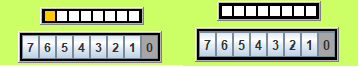
\includegraphics[scale=1]{piscapisca.png}
\caption{LED 7 alternando estados enquanto o algoritmo espera a inserção do usuário. Fonte: EdSim51}
\end{figure}
Para a inserção do usuário são envolvidas três rotinas.\newline
\textbf{Rotina "Loop-insert":} Após detectado a necessidade de \textit{input} do usuário para verificar a vitória ou a derrota, é chamada a rotina loop-insert. Ela, é responsável por detectar qualquer alteração de estado entre as chaves de SW7 à SW2, caso alguma seja pressionada, uma segunda rotina é invocada, a "Armazena-user".\newline
\textbf{Rotina "Armazena-user":} A primeira coisa que essa rotina realiza é o acendimento do LED respectivo a chave pressionada. Em seguida, se o ponteiro de memória (dado pelo registrador R0) é válido, é chamada a rotina "Salva-Usr".
\textbf{Rotina "Salva-Usr":} Rotina responsável por armazenar no local de memória dado pelo registrador R0, a chave pressionada pelo usuário.

\subsection{Comparação entre sequência aleatória e sequência do usuário}
Após realizado todo o processo de geração e salvamento de sequências, tanto aleatória quanto do usuário, o algortimo tem permissão (através de \textit{Flags}) de comparar ambas.\newline
A rotina responsável por isso é bem simples, haja vista que o algoritmo já conhece onde está salvo as duas sequências através dos registradores R0 e R1. O processo envolve comparação por meio da instrução \textbf{CJNE}, na qual, os operandos são os valores dispostos na memória entre 0x50 a 0x54 e 0x60 a 0x64. Nessa perspectiva, os valores são conferidos dois a dois, de modo que o valor presente em 0x50 seja comparado com 0x60, 0x51 com 0x61, seguindo esse passo até 0x54 e 0x64.\newline
De acordo com a funcionalidade do \textbf{CJNE}, caso os operandos sejam iguais, ele prossegue para a próxima instrução, caso contrário ele salta para uma posição de memória definida.\newline
Assim, se o usuário inseriu corretamente a sequência, ao passar por todas comparações, é chamada a rotina que escreve no LCD a mensagem \textit{Winner}. Caso o algoritmo encontre um erro na sequência é chamada a rotina que escreve no LCD a mensagem \textit{Loser!}.
Após a decisão de vitória ou derrota, o usuário pode reiniciar o jogo pressionando a chave SW0, a mesma utilizada para iniciar o jogo.
\begin{figure}[H]
\centering
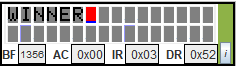
\includegraphics[scale=1]{winner.PNG}
\caption{Mensagem de vitória após comparação entre sequências. Fonte: EdSim51}
\end{figure}
\begin{figure}[H]
\centering
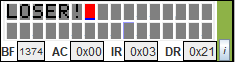
\includegraphics[scale=1]{loser.png}
\caption{Mensagem de derrota após comparação entre sequências. Fonte: EdSim51}
\end{figure}
\newpage
\section{Código fonte}
\begin{figure}[H]
\hspace*{-1.0in}
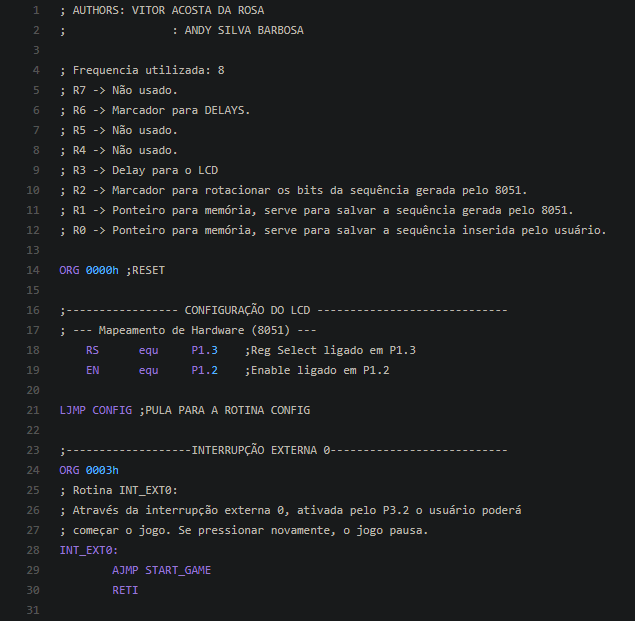
\includegraphics[scale=1]{1.png}
\end{figure}
\begin{figure}[H]
\hspace*{-1.0in}
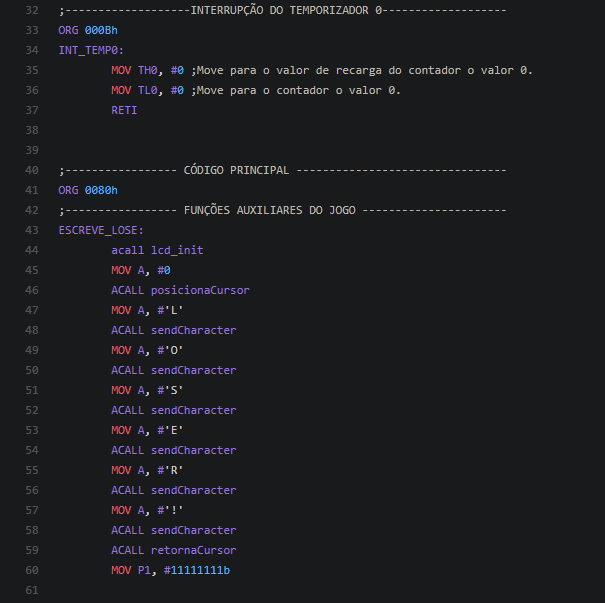
\includegraphics[scale=1]{2.PNG}
\end{figure}
\begin{figure}[H]
\hspace*{-1.0in}
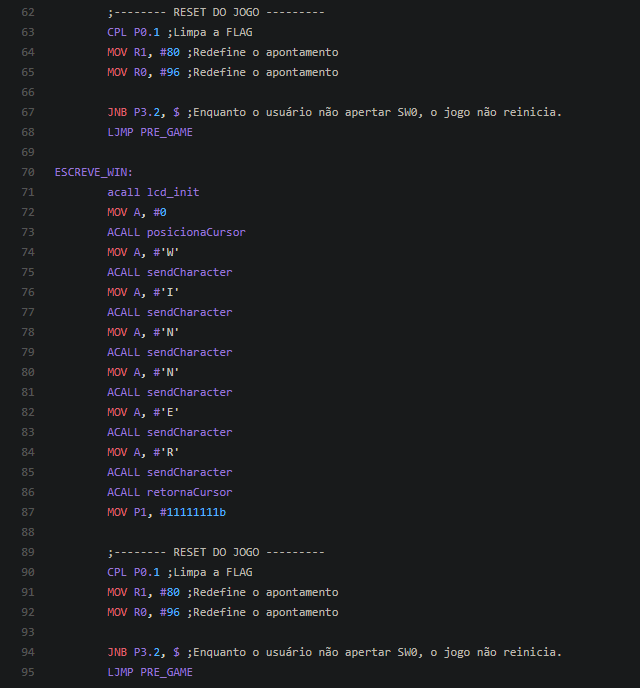
\includegraphics[scale=1]{3.PNG}
\end{figure}
\begin{figure}[H]
\hspace*{-1.0in}
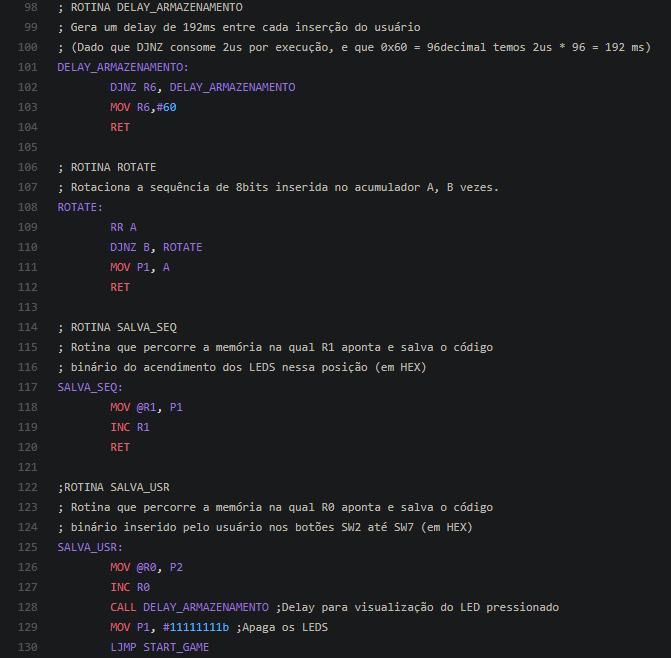
\includegraphics[scale=1]{4.PNG}
\end{figure}
\begin{figure}[H]
\hspace*{-1.0in}
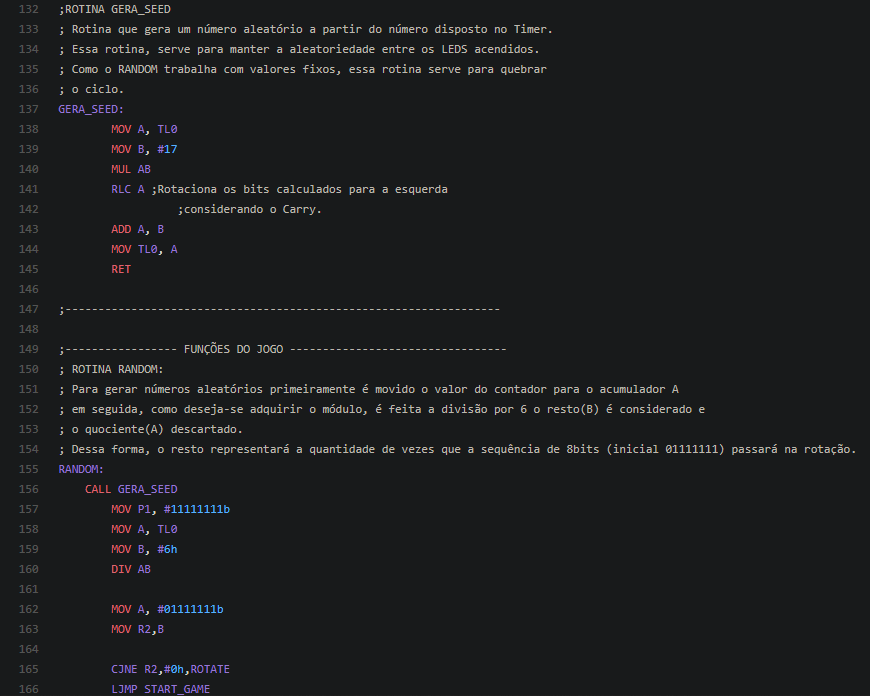
\includegraphics[scale=1]{5.PNG}
\end{figure}
\begin{figure}[H]
\hspace*{-1.0in}
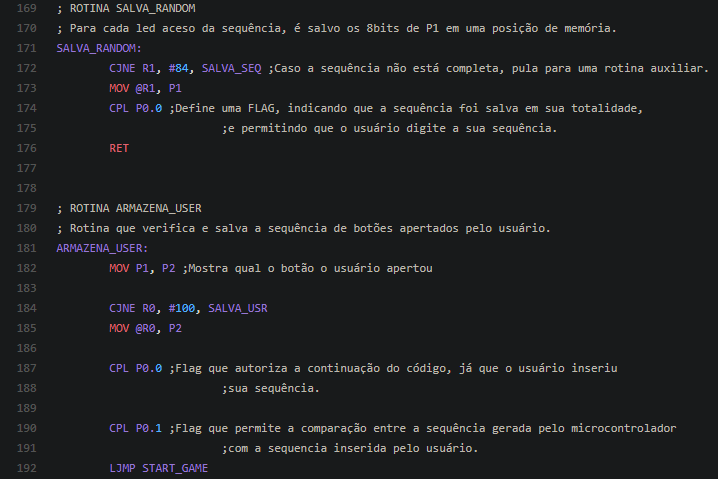
\includegraphics[scale=1]{6.PNG}
\end{figure}
\begin{figure}[H]
\hspace*{-1.0in}
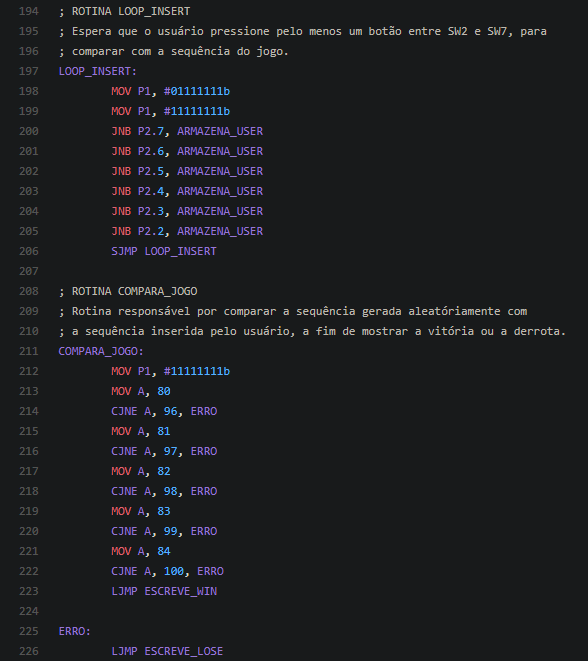
\includegraphics[scale=1]{7.PNG}
\end{figure}
\begin{figure}[H]
\hspace*{-1.0in}
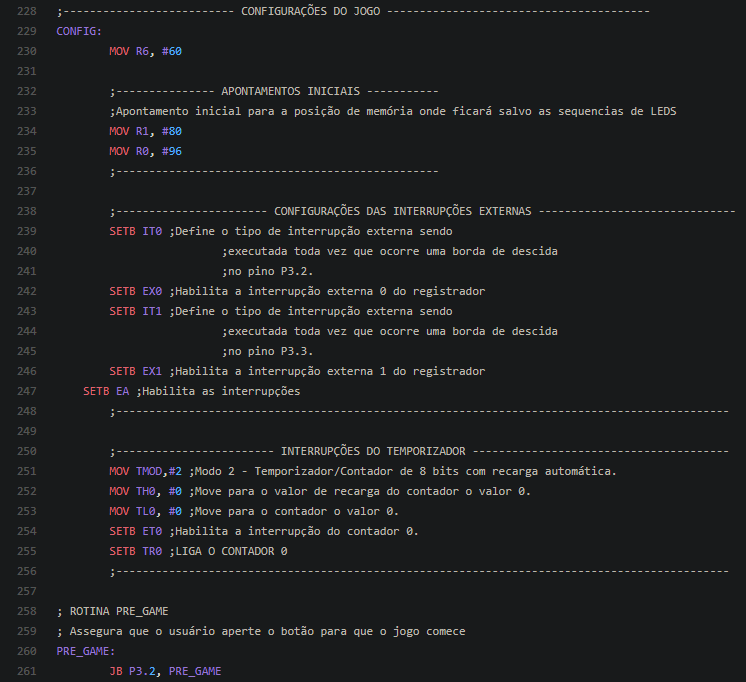
\includegraphics[scale=1]{8.PNG}
\end{figure}
\begin{figure}[H]
\hspace*{-1.0in}
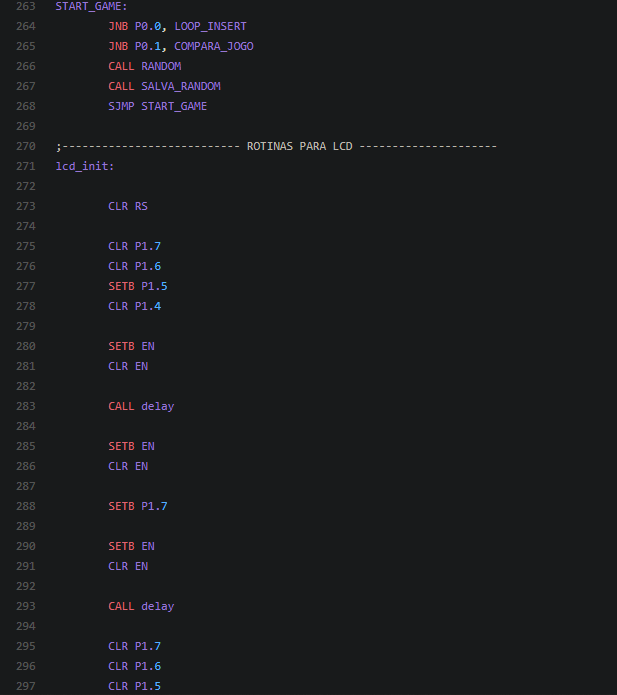
\includegraphics[scale=1]{9.PNG}
\end{figure}
\begin{figure}[H]
\hspace*{-1.0in}
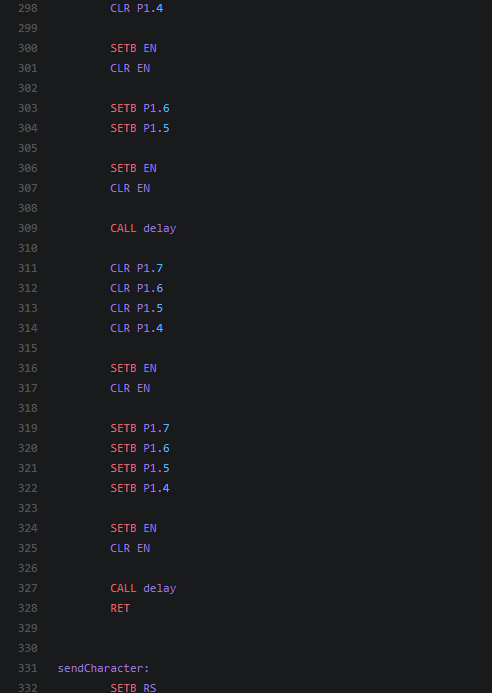
\includegraphics[scale=1]{10.PNG}
\end{figure}
\begin{figure}[H]
\hspace*{-1.0in}
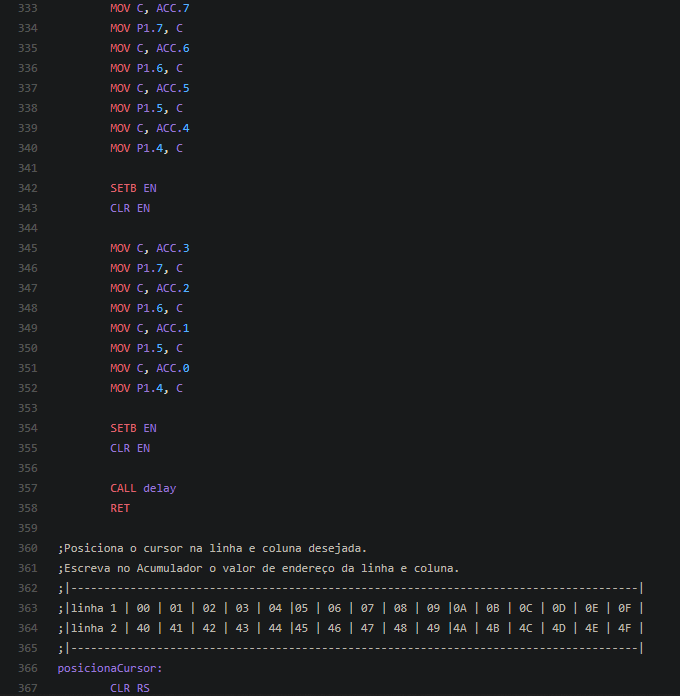
\includegraphics[scale=1]{11.PNG}
\end{figure}
\begin{figure}[H]
\hspace*{-1.0in}
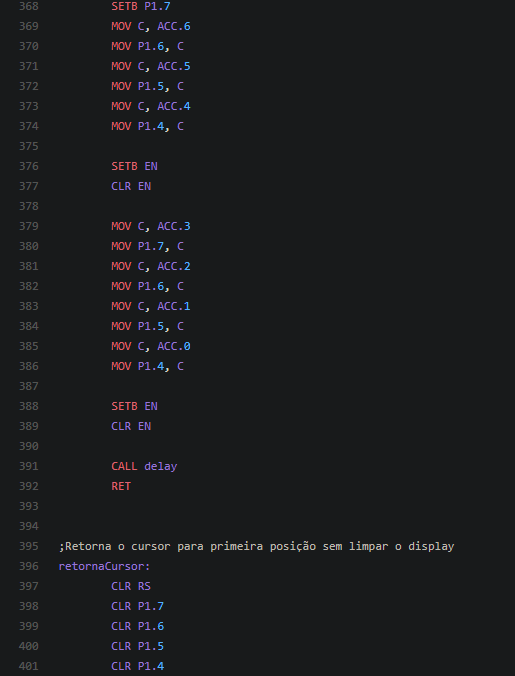
\includegraphics[scale=1]{12.PNG}
\end{figure}
\begin{figure}[H]
\hspace*{-1.0in}
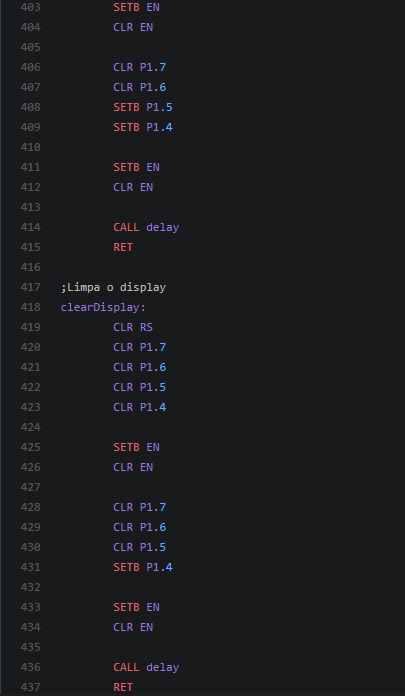
\includegraphics[scale=0.8]{13.PNG}
\end{figure}
\begin{figure}[H]
\hspace*{-1.0in}
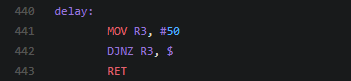
\includegraphics[scale=1]{14.PNG}
\end{figure}

\newpage
\section{Imagens da simulação realizada na IDE}
\begin{figure}[H]
\hspace*{-2in}
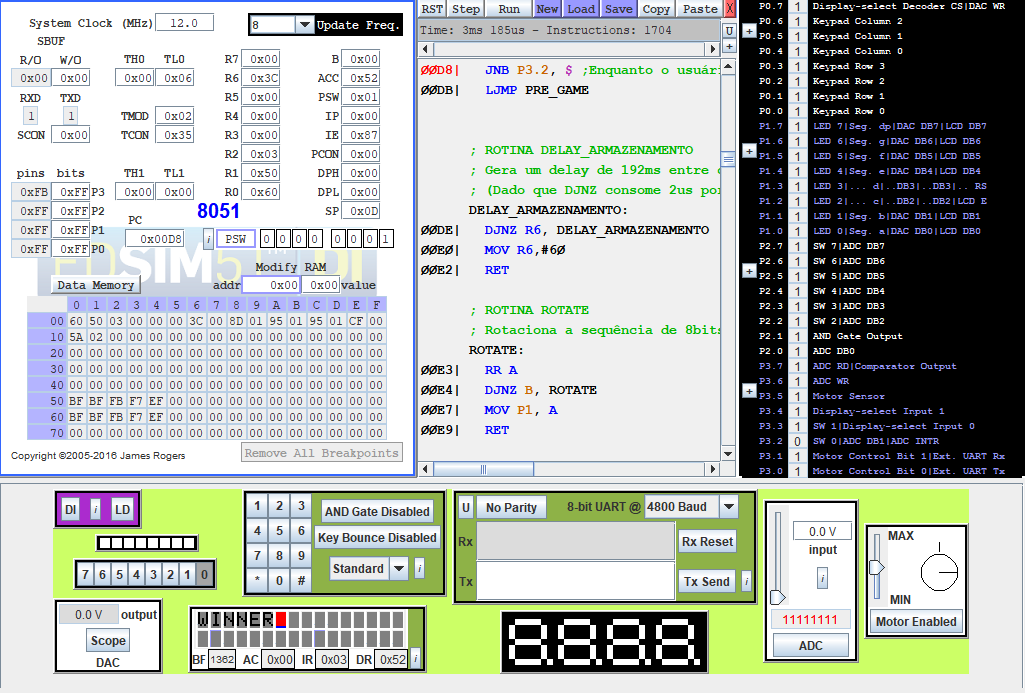
\includegraphics[scale=0.8]{vitoria.PNG}
\caption{Condição de vitória no jogo. Fonte: EdSim51}
\end{figure}
Perceba que, o conteúdo na posição de memória 0x50 é igual à 0x60, e repete-se até 0x54 e 0x64, o que indica a vitória do usuário, e o tratamento esperado.
\begin{figure}[H]
\hspace*{-2in}
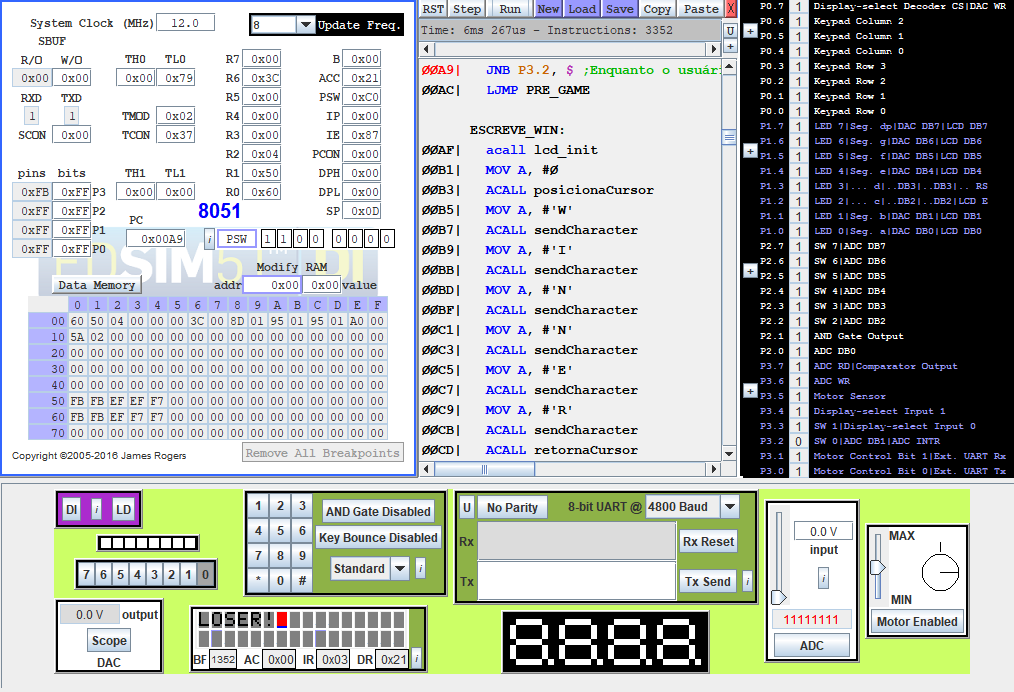
\includegraphics[scale=0.8]{perdeu.PNG}
\caption{Condição de derrota no jogo. Fonte: EdSim51}
\end{figure}
Com excessão dos valores nas posições de memória 0x53 e 0x63, todos os outros valores coincidem, na comparação, ao primeiro erro, a mensagem \textit{Loser!} será escrita, não havendo a necessidade de verificar as demais posições da memória.\newline
Perceba que entre a figura 10 e figura 11, o tempo de execução é quase o dobro, isso porque, ao terminar a escrita no LCD, o usuário pode recomeçar o jogo simplesmente apertando a chave SW0, possibilitando recomeçar indefinidas vezes.
\end{document}
